\documentclass[english]{article}
\usepackage[utf8]{inputenc}
\usepackage[a4paper, left=3cm, right=3cm, top=4cm]{geometry}

% Language & links
\usepackage[english]{babel}
\usepackage[hidelinks]{hyperref}
\usepackage{etoolbox}

% Math
\usepackage{amsmath, amsfonts, amssymb, mathtools}
\usepackage{mathrsfs}      % script letters
\usepackage{physics}       % physics notation
\usepackage{tikz-cd}       % commutative diagrams
\usepackage{amsthm}        % proof

% Figures
\usepackage{graphicx} 
\usepackage{caption}
\usepackage{subcaption}
\usepackage[table,dvipsnames]{xcolor}
\usepackage{float}

% Tables
\usepackage{array}
\usepackage{multirow}
\usepackage{colortbl}
\usepackage{hhline}
\usepackage{booktabs}
\usepackage{booktabs}
\usepackage[table]{xcolor}
\usepackage{listings}
\usepackage{xcolor}  % Optional: for custom colors
% Layout
\usepackage{tcolorbox}     % colored boxes
\usepackage{enumitem}      % custom lists
\usepackage{epigraph}      % quotes at section start
\usepackage{setspace}

% Units
\usepackage[separate-uncertainty = true]{siunitx}

% Code
\usepackage{minted}

% Appendix
\usepackage[toc]{appendix}

% Bibliography
\usepackage{csquotes}
\usepackage[backend=biber,style=numeric]{biblatex} 
\addbibresource{references.bib}

% Fix physics + siunitxW
\AtBeginDocument{\RenewCommandCopy\qty\SI}
\ExplSyntaxOn
\msg_redirect_name:nnn {siunitx}{physics-pkg}{none}
\ExplSyntaxOff

\setlength{\parindent}{0pt} % No carriage return
\onehalfspacing     % Spaziatura

\makeatletter
\def\course#1{\gdef\@course{#1}}
\def\@course{} % default value

\def\supervisor#1{\gdef\@supervisor{#1}}
\def\@supervisor{} % default value

\def\@maketitle{%
    \newpage
    \null
    \begin{center}
        % Logo
        
\includegraphics[width=1\linewidth]{img/ictp-logo.jpg}\par\vspace{1cm}
        
        % Titolo
        {\huge\scshape \@title \par}\vspace{0.5cm}
        \rule{0.7\linewidth}{0.5pt}\vspace{1cm}
    \end{center}
    
    \begin{flushright}
        {\Large\bfseries \@author \par}
        {\sffamily \@course \par}
        \vspace{0.5cm}
        {\Large Supervisor: \@supervisor \par}
        \vspace{0.5cm}
        {\Large \@date \par}
    \end{flushright}
}
\makeatother

\title{Using Closed-loop Learning as an inference device}
\author{Cerioli Gabriele}
\supervisor{Prof. Matteo Marsili}
\date{November 2025}

\begin{document}
\maketitle
\section{The algorithm}
The idea here is to use Closed-loop learning to make better estimations of the parameters of distributions.\\

For example we can consider a normal distribution with mean and variance random integers between 1 and 10.\\

The algorithm is the following:
\begin{itemize}
    \item Create a sample of $N$ points using the normal distribution with randomly generated parameters
    \item Make a Likelihood estimation of the parameters
    \item Create $M$ synthetic points from a normal distribution with the parameters estimated above
    \item Repeat this cycle with progressively larger dataset
\end{itemize}

\section{Evaluating the inference value of CLL}

We can define a metric to evaluate the usefulness of CLL in the inference.\\

If we define:
\begin{itemize}
    \item $\mu$ as the original random generated mean
    \item $\hat{\mu}$ as the mean estimated using simple Maximum Likelihood
    \item $\tilde{\mu}$ as the mean estimated after CLL cycle
\end{itemize}
and the same thing for the standard deviations.

We can define:
\begin{equation*}
    \chi_{\mu}=\frac{\left|\hat{\mu}-\mu  \right|-\left| \tilde{\mu} -\mu \right|}{\mu}
\end{equation*}
\begin{equation*}
    \chi_{\sigma}=\frac{\left|\hat{\sigma}-\sigma  \right|-\left| \tilde{\sigma} -\sigma \right|}{\sigma}
\end{equation*}

Of course if $\chi$ is negative, CLL has made our estimation of the parameter worse.\\

If we iterate this algorithm 10000 times we get the following distributions:

\begin{figure} [H]
\centering
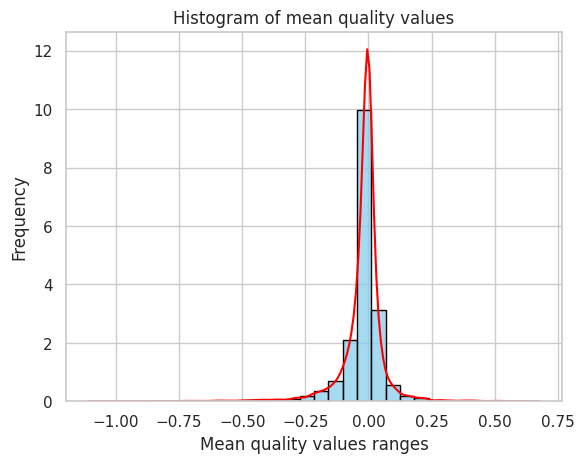
\includegraphics[width=\linewidth]{img/mean_metric.png}
\caption{Distribution of the metric for means}
\end{figure}
We can already see that the distribution is similar to a normal distribution centered at the origin.\\

The same thing is also true for the standard deviation:
\begin{figure} [H]
\centering
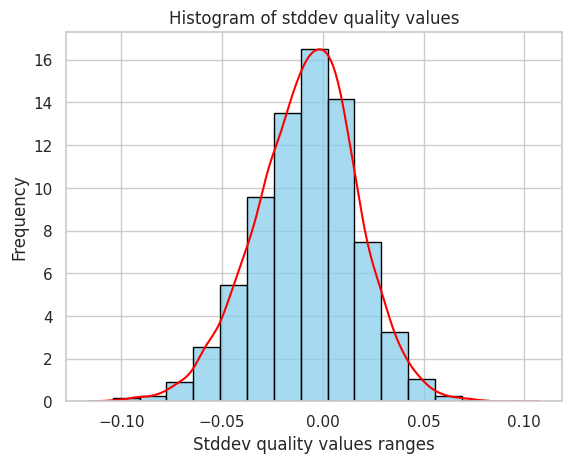
\includegraphics[width=\linewidth]{img/stddev_metric.png}
\caption{Distribution of the metric for stddev}
\end{figure}



It is also interesting to notice that the $\chi_{\mu}$ distribution has many more outliers.

\section{Conclusions}
Unfortunately by repeating the simulation multiple times the distribution are always asymmetric and centered in negative values.\\
This tells us that in this particular example using CLL does not make the estimation of the parameters better.

\end{document}